\subsection{SVM}

\paragraph{}Una máquina de soporte vectorial (SVM) es un algoritmo de aprendizaje automático supervisado utilizado fundamentalmente para problemas de clasificación.
Dado un problema de aprendizaje automático supervisado de clasificación donde las instancias del problema pueden ser clasificadas en $N$ clases y un conjunto de ejemplos de entrenamiento de dicho problema, una SVM busca encontrar un hiperplano que divida a estos ejemplos de entrenamiento de manera lineal esas $N$ clases. De esta manera, frente a una nueva instancia del problema, la SVM es capaz de clasificarla generando una correspondencia entre esta instancia y una de las $N$ clases posibles.

\paragraph{}Se denominan vectores de soporte a aquellos ejemplos de entrenamiento más cercanos al hiperplano. La distancia entre el hiperplano y un vector de soporte se conoce como márgen y, para un conjunto de ejemplos de entrenamiento, SVM busca dividirlos de manera óptima con un hiperplano donde se maximicen estos márgenes para cada uno de los vectores de soporte, cada uno asociado a su vez a una de las posibles clases de clasificación del problema. En un problema donde las instancias pueden ser clasificadas en dos clases, el hiperplano de dos dimensiones es representado por una línea recta y los vectores de soporte son aquellos ejemplos de entrenamiento más cercanos a ella, desde las dos direcciones posibles. La Figura \ref{fig:svm_margin} muestra el funcionamiento de una SVM en un problema de clasificación de dos clases.

\textsc{\begin{figure}[ht!]
	\centering
    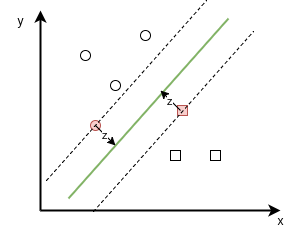
\includegraphics[width=.5\linewidth]{imagenes/svm_margenes.png}
	\caption{En esta figura se observan dos conjuntos de elementos (cuadrados y círculos), clasificados en dos clases, en base a dos características, \textit{x} e \textit{y}. El hiperplano generado por SVM se muestra como la recta negra y se marcan los márgenes en lineas punteadas. Así, en color rojo se muestran los vectores de soporte, uno perteneciente a cada clase, siendo z la distancia entre cada vector de soporte y el hiperplano.}
	\label{fig:svm_margin}
\end{figure}}


\paragraph{}El hiperplano está dado por la ecuación $g(\vec{x}) = \vec{w}^T\vec{x} + w_0$ donde $\vec{w}$ es un vector de pesos y $\vec{x}$ es el vector de características. La distancia a uno de los márgenes está dada por $z = \abs{g(\vec{x})} / \norm{\vec{w}} = 1 / \norm{\vec{w}}$, por lo que el margen total se computa como $1 / \norm{\vec{w}} +  1 / \norm{\vec{w}} = 2 / \norm{\vec{w}}$. Por lo tanto, minimizando la expresión $\norm{\vec{w}}$ se maximizan los márgenes, maximizando la separabilidad de las clases. La confianza en la clasificación de una instancia de validación, por ejemplo, está dada por la distancia de dicha instancia al hiperplano de manera directamente proporcional.

\paragraph{}Cuando se tienen más de dos clases objetivo para la clasificación, se utiliza una SVM multiclase en la cual se admiten dos posibles estrategias. Por un lado \textit{One vs. Rest} (\textit{OVR}) y por otro \textit{One vs. One} (\textit{OVO}). Dado un conjunto de $N$ clases $\{c_1,c_2,\dots,c_N\}$, \textit{OVR} intentará clasificar $c_i$ contra $\{c_1,c_2,\dots,c_{i-1},c_{i+1},\dots,c_{N - 1}\}$ dejando como representantes de la clase $C_N$ los datos que no fueron clasificados en las otras clases. Por otro lado \textit{OVO}, intentará clasificar cada clase $i$ contra cada $C_j \forall j \neq i$, creando un hiperplano para cada una de las combinaciones. Comparando las dos estrategias, \textit{OVR} genera $C_{N-1}$ clasificadores, en contraste con \textit{OVO} que genera una combinación de $N$ tomada de a dos, generando un número mayor de clasificadores que \textit{OVR}. Por otro lado, \textit{OVR} es más sensible al desbalance de los datos, en el sentido de que si se intenta clasificar y la cantidad de datos representantes de esta clase es baja en comparación con el total de datos, esta clase podría tener una ponderación o importancia mucho menor que las demás, conduciendo a una clasificación incorrecta de la instancia evaluada. En cambio, con \textit{OVO} este fenómeno no se manifiesta en igual medida, dado que se generan clasificadores uno a uno. La Figura \ref{fig:ovoovr} muestra una comparación entre estas dos estrategias.

\textsc{\begin{figure}[ht!]
	\centering
    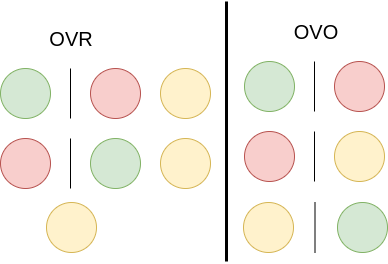
\includegraphics[width=.5\linewidth]{imagenes/ovoovr.png}
	\caption{A la izquierda se muestra la estrategia de entrenamiento de SVM \textit{OVR}, en la cual cada una de las clases se intenta clasificar contra el resto de las clases. A la derecha se muestra la estrategia \textit{OVO}, que genera clasificadores para cada par de clases.}
	\label{fig:ovoovr}
\end{figure}}

\paragraph{}La obtención de un hiperplano que divida de manera lineal a los ejemplos de entrenamiento no siempre es posible. Cuando no es posible, se suele utilizar una técnica conocida como \textit{kernelización} o \textit{Kernel Trick} para aumentar la dimensión del dominio donde se está buscando un hiperplano e intentar obtener un hiperplano que separe linealmente a los ejemplos de entrenamiento en esa dimensión. De esta manera, es posible clasificar a nuevas instancias del problema de acuerdo a este nuevo hiperplano y transformar la clasificación obtenida a la dimensión original del problema dada por las clases de clasificación disponibles. De todas maneras, una utilización imprudente del \textit{Kernel Trick} puede llevar a un sobreajuste del modelo.

\paragraph{}Entre las desventajas de utilizar SVM encontramos que los tiempos de entrenamiento asociados pueden ser significativos para grandes conjuntos de entrenamiento, pudiendo tener consumos considerables de memoria tanto durante el entrenamiento como en la validación. Así también la selección de parámetros de \textit{Kernel} para el realizar el \textit{Kernel Trick} puede ser compleja y se debe ejecutar evitando el sobreajuste.